
\section{Die Entdeckung des kosmischen Mikrowellenhintergrundes}

\chapterauthor{Yvonne Kasper, 21.12.2018}

\subsection{Theorien zur Entstehung des Universums}

Vor der Entdeckung der komischen Hintergrundstrahlung existierten insbesondere zwei verschiedene Theorien zur Entstehung des Universums.

Die erste Theorie, die sogenannte Steady State Theorie, basiert auf dem kosmologischen Prinzip.
Sie wurde insbesondere von Vertretern wie beispielsweise Albert Einstein unterstützt und geht von einer Expansion des Universums mit einer langsamen, aber kontinuierlichen Erzeugung von Materie aus. 
Hierdurch bliebe die Dichte im Universum erhalten.
Im Rahmen dieser Theorie existiert jedoch keine Erklärung für eine kosmische Hintergrundstrahlung, weshalb sie nach dessen Entdeckung 1964 von den meisten Forschern verworfen wurde.

Auf der anderen Seite existierte die Urknalltheorie, welche beispielsweise von Alexander Friedmann, Ralph Alpher oder George Gamow vertreten wurde.
Letzterer beschäftigte sich mit der Frage nach dem Ursprung der Elemente im Universum.
Hierbei sind insbesondere der Anteil von \SI{75}{\percent} Wasserstoff und \SI{24}{\percent} Helium in der interstellaren Materie zu nennen.
Nach Gamows Theorie war das Universum zu einem frühen Zeitpunkt eine heiße "Suppe" aus Protonen, Neutronen, Elektronen sowie thermaler Strahlung.
Durch Fusionsprozesse, für die hohe Temperaturen im frühen Universum von bis zu \SI{e9}{\kelvin} benötigt wurden, entsteht zunächst Deuterium aus Protonen und Neutronen und im weiteren Verlauf Helium.
Durch das Hinzufügen weiterer Protonen und Neutronen würden weitere, schwerere Elemente erzeugt werden.
Damit im Rahmen der Theorie nicht alle Protonen und Neutronen zu schwereren Kernen verschmelzen muss sich das Universum ausdehnen damit die angegebenen Fusionsprozesse durch das Ausdünnen der Materie stoppen.
Der im Rahmen dieser Theorie beschrieben "Feuerball" würde durch die Ausdehnung des Universums auf bis zu \SI{5}{\kelvin} abkühlen.
Diese Vorhersage einer kosmischen Hintergrundstrahlung wurde in einem weitgehend unbeachteten Paper von Alpher, Bethe und Gamow bereits 1948 veröffentlicht. 

\subsection{Die experimentelle Entdeckung der kosmischen Hintergrundstrahlung}

Die Physiker Robert Woodrow Wilson und Arno Allen Penzias arbeiteten ab 1963 bzw. 1962 bei den Bell Laboratories.
Zuvor beschäftigten sich beide im Rahmen ihrer Doktorarbeiten bereits mit experimentellen astrophysikalischen Themen.
Ihr neuer Arbeitgeber, die Bell Laboratories, waren ein Forschungs- und Entwicklungszentrum für die Bell Telephone Company, die US Regierung sowie die Grundlagenforschung.

Wilson und Penzias bauten eine Horn-Reflektorantenne, siehe Abbildung \ref{fig:cmb}, mit dem ursprünglichen Ziel Experimente im Bereich der Radioastronomie und Satellitenkommunikation durchzuführen. 
Ihre Antenne mit einer Länge von 15 Metern und einer \SI{6}{\metre} mal \SI{6}{\metre} großen Öffnung eignete sich gut für die Messung von schwachen Signalen.

\begin{figure}
  \centering
  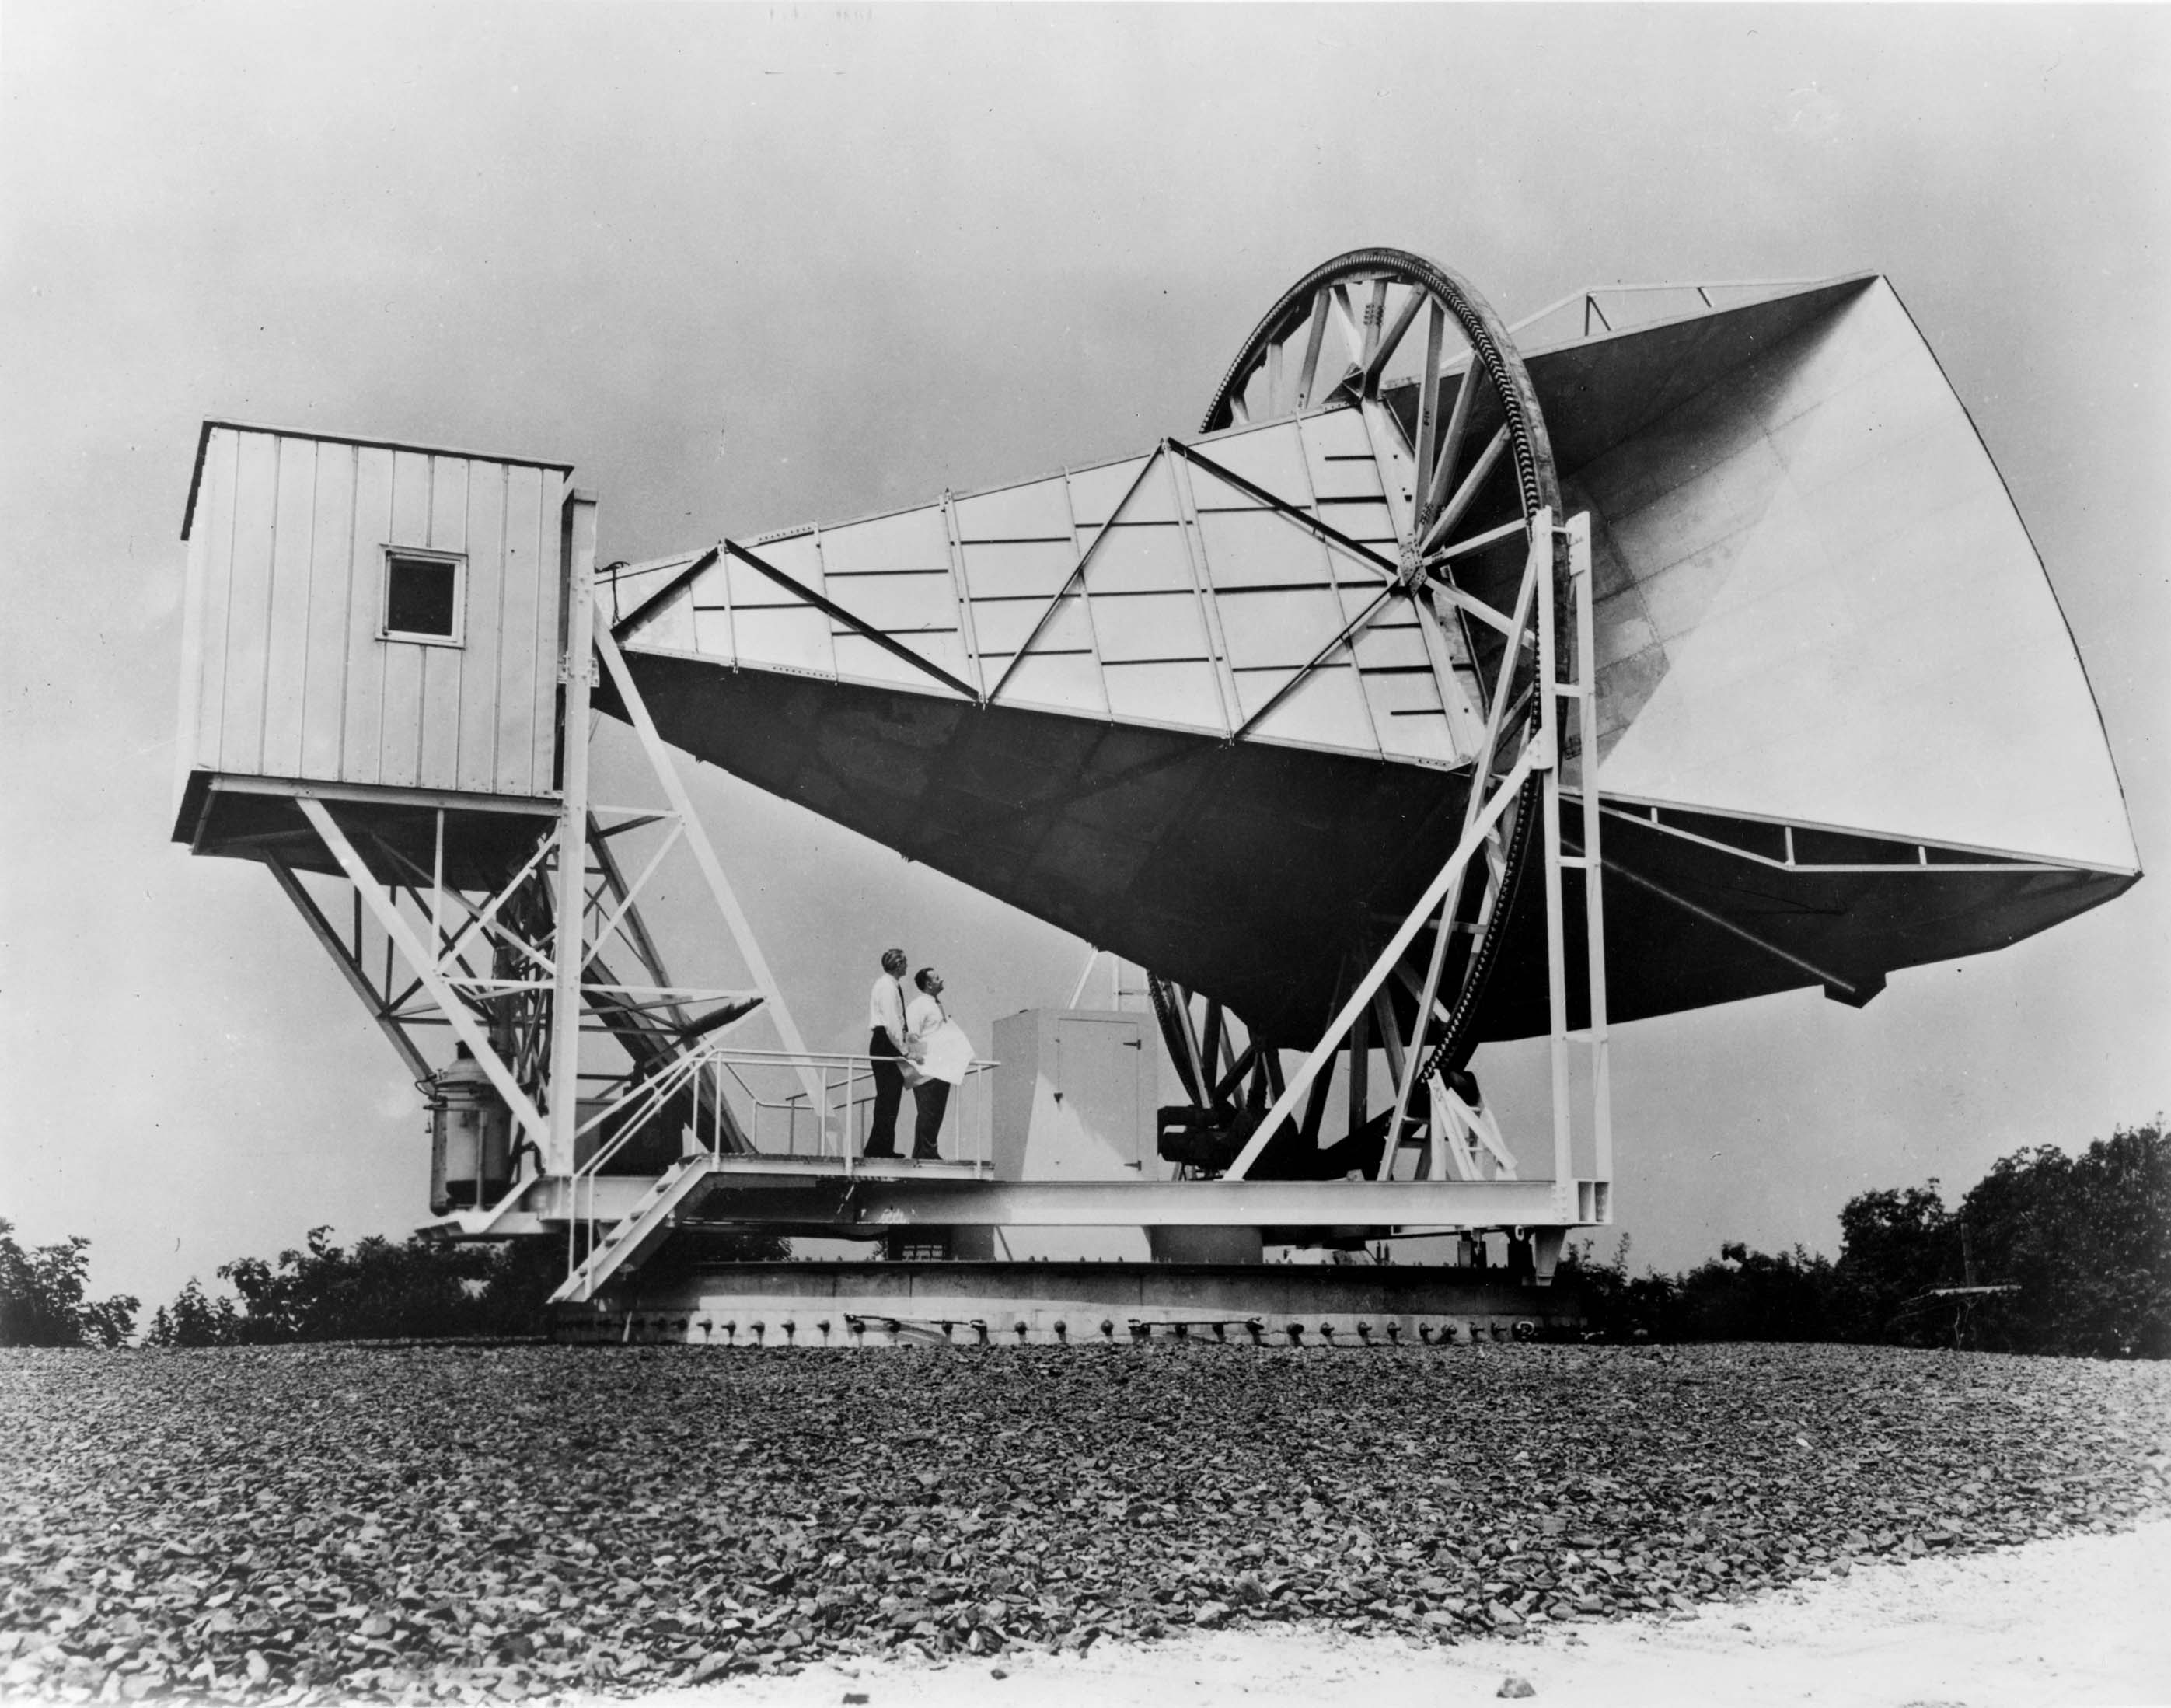
\includegraphics[height=8.0cm]{ressources/cmb.jpg}
  \caption{Von Wilson und Penzias gebaute Hornantenne mit welcher der kosmische Mikrowellenhintergrund unbeabsichtigt entdeckt wurde \cite{cmb}}
  \label{fig:cmb}
\end{figure}

Bereits erste Messungen zeigten einen unvorhergesehenen Untergrund von \SI{3.5}{\kelvin} welcher trotz mehrmonatigen Arbeiten am Empfängersystem nicht beseitigt werden konnte.
Mögliche Störungsquellen, die hierbei berücksichtigt wurden, waren beispielsweise Atmosphärenstrahlung, Störsignale der nahegelegenen Großstadt New York City, von der Regierung durchgeführte Atombombentest jedoch auch Hinterlassenschaften von Tauben in der Antenne.

Zur Interpretation der Ergebnisse sprach Penzias mit Henry Dicke aus Princton, welcher mit seiner Arbeitsgruppe bereits vorher ein ähnliches Experiment zur Untersuchung einer möglichen kosmischen Hintergrundstrahlung vorbereitet hatte.
Es wurde daraufhin von Wilson und Penzias ein Paper mit ihren experimentellen Ergebnissen sowie zeitgleich ein Paper von Dicke zur Interpretation ebendieser Ergebnisse publiziert.
Hierbei wurde der Untergrund korrekterweise als kosmische Hintergrundstrahlung interpretiert.
1978 erhielten Penzias und Wilson für ihre experimentelle Entdeckung den Nobelpreis.

\subsection{Folgende Untersuchungen der kosmischen Hintergrundstrahlung}

Nachfolgende Experimente konnten eine homogene, isotrope und unpolarisierte Hintergrundstrahlung bei ca. \SI{3.5}{\kelvin} bestätigen.
Hierzu gehörten neben erdgebundenen Experimenten auch satellitengestützte Messungen wie COBE, (W)MAP und Planck sowie Ballonexperimente wie BOOMERanG und MAXIMA.

Das COBE (Cosmic Background Explorer) Experiment untersuchte beispielsweise von 1989 bis 1993 die Infrarotstrahlung sowie hohe Frequenzen des Spektrums.
Hierbei konnte bestätigt werden, dass die kosmische Hintergrundstrahlung ein perfektes Schwarzkörperspektrum beschreibt.
Zudem wurden mit dem "Differential Microwave Radiometer" von COBE Anisotropien im CMB untersucht. 
Diese Anisotropien wurden bereits 1967 durch theoretische Berechnungen von Sachs und Wolf vorhergesagt.
Im Rahmen dieses Experimentes konnte die Temperatur des kosmischen Mikrowellenhintergrundes zu $T = \SI{2.728}{\kelvin}$ mit Temperaturfluktuationen, d.h. Anisotropien, in der Größenordnung von \num{e-5} gemessen werden.
George Smoot und John Mather erhielten für die Entdeckung dieser Anisotropien sowie dem Nachweis des Schwarzkörperspektrums 2006 den Nobelpreis.

Ein weiteres Experiment, genannt BOOMERanG (Balloon Oberservations Of Millimetric Extragalactic Radiation and Geophysics) wurde von 1998 bis 2003 in der Antarktis betrieben und konnte Messungen in bis zu \SI{42}{\kilo\metre} Höhe durchführen.
Hierbei konnten die Anisotropien in der Hintergrundstrahlung mit noch höherer Genauigkeit vermessen werden und aus diesen Ergebnissen auf die flache Geometrie des Universums geschlossen werden.

Neben dem komischen Mikrowellenhintergrund wird theoretisch auch ein Neutrinohintergrund vorhergesagt. Aufgrund der frühen Entkopplung der Neutrinos von den Elektronen und Photonen im Universum sowie dem "Reheating" des CMB, wobei durch Entropieübertrag auf die Photonen die Temperatur des Mikrowellenhintergrundes im Vergleich zum Neutrinohintergrund größer geworden ist, wird der Neutrinohintergrund bei einer Temperatur von ca. \SI{1.9}{\kelvin} vorhergesagt.
Die Messung einer solch geringen Temperatur bei Neutrios ist jedoch experimentell schwierig und war deshalb noch nicht erfolgreich.